\documentclass[12pt]{article}

%\usepackage[T1]{fontenc}
%\usepackage{merriweather}
%\usepackage{librebaskerville}
\usepackage{xcolor}
\usepackage[]{geometry}

\geometry{left=2cm,right=2cm,top=2.5cm,bottom=2cm}
\usepackage{graphicx}
\usepackage{amsfonts}
\usepackage{amsmath}
\usepackage{amssymb}
\usepackage[]{fancyhdr}
\usepackage{tikz}
\usetikzlibrary{decorations}
 \usetikzlibrary{snakes}
\begin{document}
\pagestyle{fancy}
\fancyhead[L]{\today}
\fancyhead[R]{Tomoki Goda}
%{\centering\huge On GBW model and $k_t$-factorization.}\hrule\vspace{2cm}

\section{Formula. etc}
\begin{figure}[t]
\centering
\resizebox{0.5\textwidth}{!}{
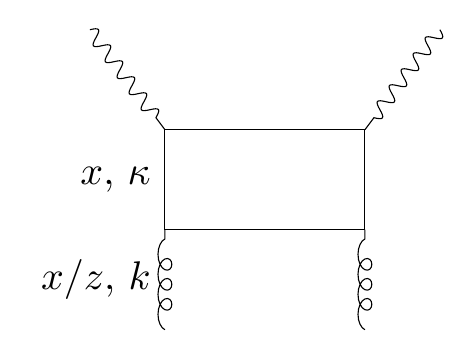
\begin{tikzpicture}
\draw[snake=coil,segment aspect=0,segment length=0.1in](-0.875in , 0.5in)--(-0.5in,0.in);
\draw[snake=coil,segment aspect=0,segment length=0.1in](0.875in ,0.5in)--(0.5in,0.in);
\draw(-0.5in , 0in)--(0.5in,0in)--(0.5in , -0.5in)--(-0.5in,-0.5in)--cycle ;
\draw(-0.5in , -0.25in)node[left,scale=0.02in]{$x$, $\kappa$};
\draw(-0.5in , -0.75in)node[left,scale=0.02in]{$x/z$, $k$};
\draw[ snake=coil,segment aspect=1.5,segment length=0.1in](0.5in , -1in)--(0.5in,-0.5in);
\draw[snake=coil,segment aspect=1.5,segment length=0.1in](-0.5in , -1in)--(-0.5in,-0.5in);
\end{tikzpicture}
}
\caption{\footnotesize Kinematic variables of gluon contribution to $\mathcal{F}$.  The momentum fraction of gluon is $x/z$ as it has to contribute via the quark box.
}
\label{fig:gluon-kinem}
\end{figure}
For protom momentum $p$ and photon momentum $q$,  define $q'\equiv q+x p$. 
Then the Sudakov decomposition of $k$ and $\kappa$ (Fig.~\ref{fig:gluon-kinem}) are
$\kappa=\alpha p-\beta q'+\kappa_t$, and $k=a p- bq'+k_t$.

Eq.~(3.9) of Kimber's thesis reads
\begin{multline}
F_2(x,Q^2)=\sum_f f_f^2 \frac{Q^2}{2\pi}\int\frac{dk^2_t}{k_t^2}\int^1_0d\beta\int d{\kappa'}_t\alpha_s \mathcal{F}(x/z,k_t^2)\Theta(1-x/z)\\
\left[\left(\beta^2+(1-\beta)^2\right)\left(\frac{I_1}{2\pi}-\frac{I_2}{2\pi}\right)
+\left(m_f^2+4Q^2\beta^2(1-\beta)^2\right)\left(\frac{I_3}{2\pi}-\frac{I_4}{2\pi}\right)\right],
\label{eq:angle-integrated}
\end{multline}
where ${\boldsymbol{\kappa}'}_t\equiv{\boldsymbol{\kappa}_t}-(1-\beta)\mathbf{k}_t$, 
\begin{equation}
\begin{split}
\frac{I_1}{2\pi}&=\frac{N_1N_2+N_3^2}{\left( N^2_1+2N_1N_2+N_3^2\right)^{3/2}}\\
\frac{I_2}{2\pi}&=\frac{N_3-(1-2\beta)N_1}{(N_1+N_4)\sqrt{ N^2_1+2N_1N_2+N_3^2}}\\
\frac{I_3}{2\pi}&=\frac{N_1+N_2}{\left( N^2_1+2N_1N_2+N_3^2\right)^{3/2}}\\
\frac{I_2}{2\pi}&=\frac{(1-\beta)}{(N_1+N_4)\sqrt{ N^2_1+2N_1N_2+N_3^2}}
\end{split}
\end{equation}
for
\begin{equation}
\begin{split}
N_1&\equiv\beta(1-\beta)Q^2+m_f^2\\
N_2&\equiv{\kappa'}_t^2+(1-\beta)^2k_t^2\\
N_3&\equiv{\kappa'}_t^2-(1-\beta)^2k_t^2\\
N_4&\equiv{\kappa'}_t^2+\beta(1-\beta)k_t^2
\end{split}
\end{equation}
and
\begin{equation}
\frac{1}{z}=1+\frac{{\kappa'}^2_t+m_f^2}{\beta(1-\beta)Q^2}+\frac{k^2_t}{Q^2}.
\end{equation}


The other formulae( %Eqs.~(3.6)~and~(3.7) of Kimber's thesis with addition of scale $\mu$ as in 
Eqs.~(3.11)~and~(3.12) of Kimber's thesis ) are,
\begin{align}
\begin{split}
F_{2T}(x,Q^2)=\sum e^2_f\frac{Q^2}{4\pi}\int\frac{d k_t^2}{k_t^2}&\int^1_0 d\beta\int d \kappa_t ^2 \frac{d\phi}{2\pi}\alpha_s(\mu^2)\mathcal{F}(x/z,k^2_t,\mu^2)\Theta(1-x/z)\\
&\left[
\left[\beta^2+(1-\beta)^2\right]
\left(\frac{\boldsymbol{\kappa}_t}{D_1}-\frac{\boldsymbol{\kappa}_t-\mathbf{k}_t}{D_2}\right)^2
+m_f^2\left(\frac{1}{D_1}-\frac{1}{D_2}\right)^2
\right]\label{eq:angle-unintegratedT}
\end{split}\\
\begin{split}
F_{2L}(x,Q^2)=\sum e^2_f\frac{Q^2}{4\pi}\int\frac{d k_t^2}{k_t^2}&\int^1_0 d\beta\int d \kappa_t ^2 \frac{d\phi}{2\pi}\alpha_s(\mu^2)\mathcal{F}(x/z,k^2_t,\mu^2)\Theta(1-x/z)\\
&\left[
4Q^2\beta^2 (1-\beta)^2\left(\frac{1}{D_1}-\frac{1}{D_2}\right)^2
\right],\label{eq:angle-unintegratedL}
\end{split}
\end{align}
where
\begin{equation}
\begin{split}
D_1&=\kappa_t^2+\beta(1-\beta)Q^2+m_f^2\\
D_2&=(\boldsymbol{\kappa}_t-\mathbf{k}_t)^2+\beta(1-\beta)Q^2+m_f^2.
\end{split}
\end{equation}
%In this case, one has additional integral of $\phi$
Except for the coupling, this is $\phi$,  the angular part of $\kappa_t$, unintegrated version of Eq.~(\ref{eq:angle-integrated}) .
The scale for $\alpha_s$ is suggested to be 
\begin{equation}
\mu^2=k^2_t+\kappa^2+m_f^2.
\label{eq:scale}
\end{equation}
Note, the integration limits of $k_t$ and $\kappa_t$ are removed as GBW gluon is not perturbative.
\section{BGK}
In order to use the GBK dipole, one needs to evaluate
\begin{equation}
\begin{split}
	\alpha \mathcal{F}(x,k_t)&=\frac{3}{4\pi}\int \frac{d^2r}{(2\pi)^2}e^{-i\mathbf{r}\cdot\mathbf{k_t}}\nabla^2_r\sigma(x,r)\\
&=\frac{3}{8\pi^2}\int dr r J_0(r k_t) \nabla^2_r\sigma(x,r).
\end{split}
\end{equation}
While $\nabla^2_r\sigma(x,r)$ is relatively smooth function, $J_0(z)$ is oscillatory function imposing difficulty in integration. Thus one may approximate  $\nabla^2_r\sigma(x,r)$.


\subsection{Alternatively...}
$\nabla^2_r\sigma(x,r)$
 of GBW is 
\begin{equation}
\sigma_0 Q_s^2 \left(1-\frac{Q_s^2}{4}r^2\right)e^{-\frac{Q_s^2}{4}r^2}.
\end{equation}
and since
\begin{equation}
	\frac{3}{4\pi} \nabla^2_r\sigma(x,r)=\int d^2ke^{-i\mathbf{r}\cdot\mathbf{k_t}}\alpha \mathcal{F}(x,k_t),
\end{equation}
small-$r$ limit is
\begin{equation}
\begin{split}
	\lim_{r\rightarrow0}\frac{3}{4\pi} \nabla^2_r\sigma(x,r)&=\pi \int^{1/r}_0 dk^2\alpha \mathcal{F}(x,k_t)\\
&=\pi \alpha xg(x,1/r).
\end{split}
\end{equation}
For this, we can propose
\begin{equation}
Q_s^2=\frac{4\pi^2 \alpha x g(x,1/r)}{3\sigma_0},
\end{equation}
which is almost BGK. 

\subsection{On running coupling of BGK}
\begin{equation}
\sigma(x,r)=\frac{4\pi}{N_c}\int\frac{d^2\mathbf{k}_t}{k_t^2}\left(1-e^{-i\mathbf{k}_t\cdot \mathbf{r}}\right)\alpha\mathcal{F}(x,k_t)
\end{equation}
in small-$r$ limit (for $k_t r\ll1$ considering large-$k_t$ region is irrelevant.), 
\begin{equation}
\begin{split}
\sigma(x,r)&=\frac{4\pi}{N_c}\int^{1/r^2}_0 dk^2_t\left(\frac{k_t^2r^2 \pi}{4}\right)\alpha\mathcal{F}(x,k_t^2)\\
&=\frac{\pi^2}{N_c}\int^{1/r^2}_0 dk^2_t \alpha\mathcal{F}(x,k_t^2)
\end{split}
\end{equation}
then in BGK,
\begin{equation}
%\begin{split}
=\frac{\pi^2}{N_c}\alpha xg(x,1/r^2).
%\end{split}
\end{equation}
But what exactly happened to $\alpha$? 
Usually the relation is 
\begin{equation}
xg(x,Q^2)=\int^{Q^2}_0 d k^2_t \mathcal{F}(x,k_t^2)
\end{equation}
without $\alpha$. 
if $\alpha=\alpha(\mu^2)$, the BGK derivation fails...
Also, note, that the argument of $\
alpha$ being $1/r$ may be a bit odd as it is not just $k^2_t$ in the $k_t$ formula.

\section{Discussion}
\subsection{Theta function, integration limits and modified $x$}
The theta function restricts
\begin{equation}
1-x\left(1+\frac{{\kappa'}_t^2+m^2}{\beta(1-\beta)Q^2}+\frac{k_t^2}{Q^2}\right)>0.
\end{equation}
Consequently, the limit $Q^2\rightarrow0$ vanishes.
It seems, it may no longer be necessary to use massive light quarks and modified $x$.

Additionally, it restricts respectively,
\begin{align}
&\frac{1-x}{x}Q^2-4m^2>k^2,\\
&\frac{1}{4} \frac{1-x}{x}Q^2-m^2>{\kappa'}_t^2,\\
&\frac{1-\sqrt{1-\frac{4m^2}{\frac{1-x}{x} Q^2  }}}{2}<\beta< \frac{1+\sqrt{1-\frac{4m^2}{\frac{1-x}{x} Q^2  }}}{2},
\end{align}
consequently
\begin{align}
1>&\frac{4m^2}{\frac{1-x}{x} Q^2 }&& \rightarrow& x&<\frac{1}{1+\frac{4m^2}{Q^2}}.
\end{align}
That is, 
\begin{equation}
x_{m}<1.
\end{equation}
Now, considering that $x_m$ was $x$ of GBW gluon $\mathcal{F}(x,k^2)$, $x/z<1$ and the treatment of GBW with $x_m$ seem to correspond to each other.

\subsection{Which formula(e) to be used.}
Eq.~(\ref{eq:angle-integrated}) is relatively straight forward to implement, and \underline{\textbf{currently used}}. \\
Eqs.~(\ref{eq:angle-unintegratedT})~(\ref{eq:angle-unintegratedL}) are more difficut due to the additional angular integral. However, it is necessary should one intend to use the running coupling with argument suggested in Kimber's formula (Eq.~(\ref{eq:scale})).
\subsection{Preliminary data}
\begin{figure}
\includegraphics[width=0.5\textwidth]{./preliminary.png}
\includegraphics[width=0.5\textwidth]{./preliminary-dipole.png}
\caption{\footnotesize Preliminary result for \underline{\textbf{selected}} combinations of \{fixed $\alpha_s$ (``fix"), running $\alpha_s$ (``run")\}  $\otimes$ \{ modified $x$ (``mod"), Bjorken $x$ (``Bjor")\}  $\otimes$ \{$\sigma_\mathrm{dipole}$ formula (``r"), $\mathcal{F}$ formula (``")\}.
By running, it does not mean using Eqs.~(\ref{eq:angle-unintegratedT})~(\ref{eq:angle-unintegratedL}), but simply multiplying GBW $\mathcal{F}$ by $\frac{ \alpha(\mu^2) }{0.2}$, where $\alpha(\mu^2)=\frac{1}{b_0 \log\left(\frac{\mu^2}{\Lambda_\mathrm{QCD} }\right)}$ and $\mu^2=\max( k^2_t+{\kappa'}_t^2+m_f^2,2\Lambda_\mathrm{QCD})$. (!!NOTE!!, it is ${\kappa'}_t$ being used here, not $\kappa_t$ as in the Kimber's formula ! (cf. Eq.~(\ref{eq:scale})).\\
Left:$ \alpha_s\mathrm{F}$, Right: $\sigma/\sigma_0$. (note, it is not $\alpha_s(\mu^2)$ for running case when plotted.) $Q^2=100\mathrm{GeV^2}$, $x=10^{-4}$.
}
\end{figure}

\begin{itemize}
\item all comparable $\chi^2 $. 
\begin{itemize}
\item $\alpha, x_m\;\sim5.4$, 
\item $\alpha, x_B\;\sim4.4$,
\item $\alpha, x_m, r\;\sim4.4$, 
\item $\alpha(\mu), x_B\;\sim4.0$
\end{itemize}
$\rightarrow$ modification of $x$ is worsening.
Later shown, theta function should deal with the photo production. There may not be necessity any more.\\
\item most noteble difference is $\sigma_0$
\begin{itemize}
\item $\alpha, x_m\;\sim32$, 
\item $\alpha, x_B\;\sim33$,
\item $\alpha, x_m, r\;\sim19$, 
\item $\alpha(\mu), x_B\;\sim44$
\end{itemize}
$\rightarrow$ Generally the $k_t$ versions have much higher $\sigma_0$.
Note, Massive light quarks case has higher $\sigma_0$. Probably due  to the suppression by $x(1+4m^2/Q^2)$.

\section{Concluding Remarks}
\begin{itemize}
\item modified $x$ deteriorates the fit while there is no longer apparent necessity.
\item Even with incorrect(?) incorporation of $\alpha_s(\mu)$, it has positive effect on the fit. 
\item biggest difference in the fit paramaeters is the normalization $\sigma_0$. 
\end{itemize}
\end{itemize}

\section{Code, technicality}
The fitting program has been rewritten completely in order to accommodate C++  Minuit2 and OOP. \\
The repository is \\
\textit{ git@github.com:Tomoki-Goda/Saturation-Model.git }\\
At the early stage of development the integrations were done with private implementations of Gauss-Legendre quadrature, Curtis-Clenshaw quadrature, or CERNLIB subroutines(mostly DGAUSS). 
These functions (mostly the Clensaw-Curtis function is used for speed and flexibility) are not very tolerant for step by the theta function. Besides, the Clenshaw method has to take end points of the integration region, making it unsuitable for cases where integrand is numerically ill defined at the end points.
Cuba package has been implemented. Cuhre works similar to previous versions in terms of performance (except for possiblly better handling of failure). Vegas and Suave takes too long (possibly not optimized). 

\section{Changes of variables}
For $x=[0,1]$ and $y=[a,b]$, one can use following changes of variables:
\begin{align}
y&=b x+a(1-x), \\
y&=a\left(\frac{b}{a}\right)^x,\\
y&=\frac{a(b-a)(1-x)+x b}{(b-a)(1-x)+x}.
\end{align}
Note, only the third one can be used for $a=0, b=\infty$, where $y=\frac{x}{1-x}$.

Then using this, 
\begin{equation}
\int^u_l dy f(y)=\int^1_0 \left(\frac{dy}{dx}\right) dx f(y(x;l,u)).
\end{equation}
For a multidimensional case, one may have
\begin{equation}
\begin{split}
\int^{u_1}_{l_1} dy_1\int^{u_2}_{l_2} dy_2 f(y_1,y_2)& \Theta(\dots)\\
=\int^1_0\int^1_0& \left(\frac{\partial y_1}{\partial x_1}\right) \left(\frac{\partial y_2}{\partial x_2}\right)dx_1 dx_2 f\left(y_1(x_1; l ,u ),y_2(x_2; l_2(x_1) ,u_2(x_1 ) )\right).
\end{split}
\end{equation}
\section{Peak}
Ignoring the theta function, and if we take limits $m_f^2\rightarrow0,\;\beta\rightarrow0$, 
the donominators of $I_i$, $N_1^2+2N_1N_2+N_3^2\rightarrow {\kappa'}_t^2-k_t^2$.
that is, when $\beta$ is small , one has a ridge at ${\kappa'}_t^2=k_t^2$ (We never actually hit the singular point as thetha function restrict lower limit of $\beta$. ).

When there is a integrable peak at $x\sim0$ of $[0,1]$, one may use $x\rightarrow {x'}^2$. 
consider when integrating 
\begin{equation}
\frac{1}{\sqrt{(x_1-x_2)^2}+\epsilon},
\end{equation}
for small $\epsilon$.
 then one use
\begin{align}
x_1 &\rightarrow (1-{x'}_1) x_2& x_2 &\rightarrow (1-{x'}_2) x_1
\end{align}
then
\begin{align}
x_2&\frac{1}{ ({x'}_1 x_2)+\epsilon}& x_1&\frac{1}{({x'}_2 x_1)+\epsilon}
\end{align}



\section{Connection to the momentum space formula}
Firstly, let us conider 
\begin{align}
&\left(\frac{1}{D_1}-\frac{1}{D_2}\right)^2&
&\text{and}&
&\left(\frac{\boldsymbol{\kappa}_t}{D_1}-\frac{\boldsymbol{\kappa}_t-\mathbf{k}_t}{D_2}\right)^2
\end{align}
of Eqs.~(\ref{eq:angle-unintegratedT})~and~(\ref{eq:angle-unintegratedL}).

Using identities (demonstrated at the end of the section), 
\begin{align}
\begin{split}
\left(\frac{1}{\kappa_t^2+N_i^2}-\frac{1}{(\boldsymbol{\kappa}_t-\mathbf{k}_t)^2+N_i^2} \right)&\\
=-i &\left( 
\int\frac{d^2\mathbf{r}}{2\pi}e^{i \boldsymbol{\kappa}_t\cdot\mathbf{r}}K_0(N_1 r)
- \int\frac{d^2\mathbf{r}}{2\pi}e^{i (\boldsymbol{\kappa}_t-\mathbf{k}_t)\cdot\mathbf{r}}K_0(N_1 r)
\right)
\end{split}\\
\begin{split}
\left(\frac{\boldsymbol{\kappa}_t}{\kappa_t^2+N_i^2}-\frac{\boldsymbol{\kappa}_t-\mathbf{k}_t}{(\boldsymbol{\kappa}_t-\mathbf{k}_t)^2+N_i^2} \right)&\\
=-i N_1& \left( 
\int\frac{d^2\mathbf{r}}{2\pi}\left(\frac{\mathbf{r}}{r}\right)e^{i \boldsymbol{\kappa}_t\cdot\mathbf{r}}K_1(N_1 r)
- \int\frac{d^2\mathbf{r}}{2\pi}\left(\frac{\mathbf{r}}{r}\right)e^{i (\boldsymbol{\kappa}_t-\mathbf{k}_t)\cdot\mathbf{r}}K_1(N_1 r)
\right)
\end{split}
\end{align}
And multipying by complex conjugate ({\color{red} Nowhere it is mentioned that it is complex conjuagte, but following Kowalski, it seems like so.})
\begin{align}
\begin{split}
\left(\frac{1}{D_1}-\frac{1}{D_2}\right)^2&\\
&=\int\frac{d^2\mathbf{r}}{2\pi}\int\frac{d^2\mathbf{r}'}{2\pi}
e^{i \boldsymbol{\kappa}_t\cdot(\mathbf{r}-\mathbf{r}')}
 \left(1 -e^{-i\mathbf{k}\cdot \mathbf{r}}
\right)
\left(1 -e^{i\mathbf{k}\cdot \mathbf{r}'}
\right)
K_0(N_1 r)K_0(N_1 r')
\end{split}\\
\begin{split}
\left(\frac{\boldsymbol{\kappa}_t}{D_1}-\frac{\boldsymbol{\kappa}_t-\mathbf{k}_t}{D_2}\right)^2&\\
=&\int\frac{d^2\mathbf{r}}{2\pi}\int\frac{d^2\mathbf{r}'}{2\pi}
\left(\frac{\mathbf{r}\cdot\mathbf{r}'}{r r'}\right)
e^{i \boldsymbol{\kappa}_t\cdot(\mathbf{r}-\mathbf{r}')}
 \left(1 -e^{-i\mathbf{k}\cdot \mathbf{r}}
\right)
\left(1 -e^{i\mathbf{k}\cdot \mathbf{r}'}
\right)
K_1(N_1 r)K_1(N_1 r')
\end{split}
\end{align}
Now,  if \underline{\color{blue} one assumed that $x/z$ and $\mu$ have no dependence on $\kappa_t$,} one can integrate over $\boldsymbol{\kappa}_t$ to yield a delta function $(2\pi)^2 \delta^2(\mathbf{r}-\mathbf{r}')$.\\
Thus obtains,
\begin{align}
\int \frac{d^2\boldsymbol{\kappa}_t}{2\pi}\left(\frac{1}{D_1}-\frac{1}{D_2}\right)^2
&=\int\frac{d^2\mathbf{r}}{2\pi}
\left |1 -e^{i\mathbf{k}\cdot \mathbf{r}}
\right|^2
K_0^2(N_1 r)
\\
\int \frac{d^2\boldsymbol{\kappa}_t}{2\pi}\left(\frac{\boldsymbol{\kappa}_t}{D_1}-\frac{\boldsymbol{\kappa}_t-\mathbf{k}_t}{D_2}\right)^2&
=\int\frac{d^2\mathbf{r}}{2\pi}
\left|1 -e^{i\mathbf{k}\cdot \mathbf{r}}
\right|^2
K_1^2(N_1 r).
\end{align}
Inserting back to Eqs.~(\ref{eq:angle-unintegratedT})~and~(\ref{eq:angle-unintegratedL}) (angular part of $\mathbf{k}_t$ is brought back),
\begin{align}
\begin{split}
F_{2T}(x,Q^2)=2\sum e^2_f\frac{Q^2}{4\pi^2}\int^1_0 d\beta\int\frac{d^2\mathbf{r}}{2\pi}
{\color{blue}\int\frac{d^2 \mathbf{k}_t}{k_t^2} \alpha_s(\mu^2)\mathcal{F}(x/z,k^2_t,\mu^2)\left |1 -e^{i\mathbf{k}\cdot \mathbf{r}}
\right|^2
}
&\Theta(1-x/z)\\
\times
\Big[
\left[\beta^2+(1-\beta)^2\right]
K_0^2(N_1 r)+&m_f^2
K_1^2(N_1 r)
\Big]
\end{split}\\
\begin{split}
F_{2L}(x,Q^2)=2\sum e^2_f\frac{Q^2}{4\pi^2}\int^1_0 d\beta \int\frac{d^2\mathbf{r}}{2\pi}
{\color{blue}\int\frac{d^2 \mathbf{k}_t}{k_t^2}
\alpha_s(\mu^2)\mathcal{F}(x/z,k^2_t,\mu^2)\left|1 -e^{i\mathbf{k}\cdot \mathbf{r}}
\right|^2
}
&\Theta(1-x/z)\\
\times
\Big[
4Q^2\beta^2 (1-\beta)^2&
K_1^2(N_1 r)
\Big].
\end{split}
\end{align}
Using the familiar equation
\begin{equation}
\sigma(x,r)=\frac{2\pi}{3}\int\frac{d^2\mathbf{k}}{k^2}\alpha\mathcal{F}(x,k^2)\left|1-e^{i \mathbf{k}\cdot\mathbf{r}}\right|,
\end{equation}
\underline{\color{blue}and again, assuming $z$ and $\mu$ are independent of $k_t$,}
\begin{align}
\begin{split}
F_{2T}(x,Q^2)=6\sum e^2_f\frac{Q^2}{4\pi^2}\int^1_0 d\beta\int\frac{d^2\mathbf{r}}{(2\pi)^2}
\sigma(x/z,r)
&\Theta(1-x/z)\\
\Big[
\left[\beta^2+(1-\beta)^2\right]&
K_0^2(N_1 r)
+m_f^2
K_1^2(N_1 r)
\Big]
\end{split}\\
\begin{split}
F_{2L}(x,Q^2)=6\sum e^2_f\frac{Q^2}{4\pi^2}\int^1_0 d\beta \int\frac{d^2\mathbf{r}}{(2\pi)^2}
\sigma(x/z,r)
&\Theta(1-x/z)\\
\Big[&
4Q^2\beta^2 (1-\beta)^2
K_1^2(N_1 r)
\Big].
\end{split}
\end{align}
{\color{red} Factor of $(2\pi)^2$ different from the GBW.} (and of course  $x\leftrightarrow x/z$.)

\textbf{\color{blue}\underline{ One then identifies that GBW formula is obtained assuming $ 1/z=\left(1+4 m_f^2/Q^2\right)$.}}\\
This corresponds to $k_t,\kappa'_2\sim0$ and $\beta\sim 1/2$. This assumption makes it necessary to have massive light quarks to replace non-zero $k_t$ and $\kappa'_2$.
{\color{green} We didn't need to assume anything about $\beta$. can't we use for $x_\mathrm{mod}$ ?}\\

{\Large Therfore, modified $x$ is unnecessary for $k_t$ formula !!}

\subsection{The identities}
For $i=1,2$.
The identity can be demonstrated as follows.
Starting from
\begin{equation}
i N_1^j\int\frac{dr d\theta}{2\pi} r\left( \frac{\mathbf{r}}{r}\right)^j e^{i r k \cos\theta}K_j(N_1 r),
\end{equation}
where $j=0,1$.
One decompose in $\hat{\mathbf{k}}$ and $\hat{\mathbf{k}'}$, where $\hat{\mathbf{k}}\cdot \hat{\mathbf{k}'}=0$. 
Then 
\begin{equation}
=i N_1^j\int\frac{dr d\theta}{2\pi}r \left(\frac{r\left( \hat{\mathbf{k}} \cos\theta+\hat{\mathbf{k}'}\sin\theta\right)}{r}\right)^j  e^{i r k \cos\theta}K_j(N_1 r).
\end{equation}
Since the integration over $\theta$ for the $\sin\theta$ term is 0,
\begin{equation}
=i N_1^j \hat{\mathbf{k}}^j\int\frac{dr d\theta}{2\pi}r \left(  \cos\theta \right)^j  e^{i  r k \cos\theta}K_j(N_1 r).
\end{equation}
Using, 
\begin{equation}
\int^\pi_{-\pi}\cos(j \theta)e^{\pm i z \cos(\theta)}=\pm 2\pi i J_j(z),
\end{equation}
and keepng in mind $j=0,1$ only,
\begin{equation}
\begin{split}
=i N_1^j \hat{\mathbf{k}}^j\int\frac{dr d\theta}{2\pi} r  \left( \cos (j \theta)\right) e^{i rk \cos\theta}K_j(N_1 r)\\
=- N_1^j \hat{\mathbf{k}}^j\int^\infty_0 dr r J_j(kr )K_j(N_1 r)
\end{split}
\end{equation}
Lastly, using
\begin{equation}
\int^\infty_0 dr r J_j(r k) K_j( r N_1)=\left(\frac{|k|}{N_1}\right)^j\frac{1}{k^2+N_1^2},
\end{equation}
one arrives to the identity
\begin{align}
i N_1\int\frac{d^2\mathbf{r}}{2\pi} \left( \frac{\mathbf{r}}{r}\right) e^{i r k \cos\theta}K_1(N_1 r)&=-\mathbf{k} \frac{1}{k^2+N_1^2}\\
i \int\frac{d^2\mathbf{r}}{2\pi}e^{i r k \cos\theta}K_1(N_1 r)&=- \frac{1}{k^2+N_1^2}
\end{align}
{\color{red} Somehow there is a sign difference from the Kowalski's paper. For now, trivial.}



\section{Log rise...}
\begin{equation}
\alpha \mathcal{F} =\frac{3}{8\pi^2}\int^\infty_0dr r J_0(r k)\nabla^2_r \sigma
\end{equation}
in small $k$ limit,
\begin{equation}
\begin{split}
\lim_{k\rightarrow0 } \alpha \mathcal{F} &=\frac{3}{8\pi^2}\int^\infty_0dr r \nabla^2_r \sigma\\
&=\frac{3}{8\pi^2}\int^\infty_0dr r\left[\frac{\partial^2\sigma}{\partial r^2}+\frac{\partial\sigma}{\partial r}\right]\\
&=\frac{3}{8\pi^2}\left[r\frac{\partial\sigma}{\partial r}-\int dr \frac{\partial\sigma}{\partial r} +\sigma \right]^\infty_0\\
&=\frac{3}{8\pi^2}\left[r\frac{\partial\sigma}{\partial r}\right]^\infty_0=\frac{3}{8\pi^2}\left[\frac{\partial\sigma}{\partial \log(r)}\right]^\infty_0
\end{split}
\end{equation}

\begin{figure}
\includegraphics[width=\textwidth]{./dipole1.png}
\caption{Dipole cross sections. Left: GBW, Right: BGK.}
\end{figure}
\begin{figure}
\includegraphics[width=\textwidth]{./gluon1.png}
\caption{Observe the new structure arizing from the DGLAP (larger-$k_t$ peak). When $x$ is small it becomes the dominant contributon. Also there is a narrow ridge around $x\sim1$. It is probably a saturation line, i.e. the line is not straight like in GBW case. {\color{green}Some change of variables may be helpfull...}   }
\end{figure}


\section{Computational strategies}
\subsection{$\alpha\mathcal{F}$ and $\nabla^2_r \sigma$}
\begin{equation}
\begin{split}
\alpha\mathcal{F}&=\frac{3}{8\pi^2}\int^\infty_0dr r J_0(r k)\nabla^2_r \sigma(x,r)\\
&=\frac{3}{8\pi^2}\int^\infty_0dr rJ_0(r k) \left(\frac{1}{r}\frac{\partial}{\partial r}\left(r\frac{\partial}{\partial r}\right)\right) \sigma(x,r)
\end{split}
\end{equation}
Using integration by parts,
\begin{equation}
\begin{split}
\alpha\mathcal{F}&=\frac{3}{8\pi^2}\int^\infty_0dr J_0(r k) \frac{\partial}{\partial r} \left(r\frac{\partial}{\partial r}\right) \sigma(x,r)\\
&=\frac{3}{8\pi^2}\left[ J_0(r k)\left(r\frac{\partial}{\partial r}\right) \sigma(x,r) - \int dr \frac{\partial J_0(r k)}{\partial r} \left(r\frac{\partial}{\partial r}\right) \sigma(x,r)\right]^\infty_0\\
&=\frac{3}{8\pi^2}\left[  \int dr r k J_1(r k)\frac{\partial}{\partial r}\sigma(x,r)\right]^\infty_0,
\end{split}
\end{equation}
assuming 
\begin{equation}
\lim_{r\rightarrow0,\infty}J_0(r k)\left(r\frac{\partial}{\partial r}\right) \sigma(x,r)=0.
\end{equation}
Hence, one has two ways to compute the gluon density;
\begin{align}
&\frac{3}{8\pi^2}\int^\infty_0dr r J_0(r k)\nabla^2_r \sigma(x,r)\\
&\frac{3}{8\pi^2}\int^\infty_0  dr r k J_1(r k)\frac{\partial}{\partial r}\sigma(x,r)
\end{align}
Now, these integrals are in the form of\textbf{ Hankel transform}.

as a by-product of interpolation, derivatives are obtainable in gsl\_cheb or gsl\_interp. However in any case second derivative may become a source of inaccuracy...


Let us assume small $Q_s^2$, and for $r>>Q_s$, integrand is negligible, then
\begin{equation}
\begin{split}
\frac{3}{8\pi^2}\int^{1/Q_s}_0  dr r k J_1(r k)\frac{\partial}{\partial r}\sigma(x,r)\\
\simeq \frac{3}{8\pi^2}\int^{1/Q_s}_0  dr  k J_1(r k) r^2 Q_s^2\\
=\frac{3Q_s^2}{8\pi^2} \frac{J_2(k/Q_s)}{k Q_s^2}  
\end{split}
\end{equation}



\end{document}